\section{The Software Out-of-Order Processor}
\label{sec:soop}

There are two major challenges in implementing an efficient task
scheduler for Legion:
\begin{itemize}
\item  For correctness, Legion must guarantee that every pair of {\em dependent} tasks is serialized in program order.

\item For performance, Legion must hide the extremely long latencies associated
  with machines that have both distributed memory and many levels of
  memory hierarchy.
\end{itemize}
Our scheduler uses three techniques to achieve both correctness and high performance:
\begin{itemize}
\item If it were necessary to compare all pairs of tasks for dependences that 
would be a bottleneck in most Legion programs.  Fortunately,
subtasks enjoy an isolation property that allows Legion to check only task siblings for dependences
(see Section~\ref{sec:dep}).

\item Legion uses a {\em  software out-of-order processor}, or SOOP, to schedule tasks.  The SOOP 
is pipelined and distributed, and also extracts nested parallelism from subtasks.

\item Legion uses a {\em deferred execution model} that decouples the issuing
of operations from when operations are performed.  An issued operation waits for other operations on
which it is dependent to complete before executing, but a waiting operation does not cause the SOOP
to block, allowing Legion to perform other useful work while the operation is pending.  

%  For example, Legion may issue a copy
%operation to move the results of a task $a$ to the place where a task $b$ will take the copied data as
%an argument.  Tasks $a$ and $b$ and the copy can all be issued, but the copy will not start until
%task $a$ completes and task $b$ will not start until the copy completes.

\end{itemize}

Each processor in the machine runs an instance of the SOOP, which handles all requests
for Legion services from tasks executing on the processor.  The SOOP is analagous to the out-of-order
instruction scheduler in superscalar processors, but working at the granularity of tasks and their region
arguments instead of instructions and their register arguments.
Legion's SOOP has a five stage pipeline: dependence analysis (Section~\ref{sec:dep}),
distribution (Section~\ref{sec:dist}),
mapping (Section~\ref{sec:map}),
execution (Section~\ref{sec:exec}),
and clean-up (Section~\ref{sec:clean}).
We discuss each stage in turn.

\subsection{Depedence Analysis}
\label{sec:dep}


When a Legion task runs, it may spawn new subtasks to be executed.  We refer to the
subtasks as {\em children} of the {\em parent} task.  The children of a parent task
are {\em siblings} of each other.  A task always executes on a single processor, but
its subtasks may execute elsewhere.

When a parent task spawns a child task, the child is {\em registered}
with the SOOP on the processor where the parent is executing;
registration records the subtask's logical region arguments and
associated privileges and coherence properties.  Children are
registered in the sequential execution order in which the parent task
spawns them and enqueued for dependence analysis.  For example, in the
circuit simulation in Listing~\ref{lst:code_ex}, the three spawn
statements on lines 32-34 register will register all of the three
kinds of subtasks (in program order) on the processor where {\tt
simulate\_circuit} executes.

If two children have a dependence between their region arguments, the
SOOP will schedule them to run serially to preserve the program's
sequential semantics.  If two child tasks have no dependence then
Legion can schedule them to execute out of order, in parallel.  Thus,
the first stage in the execution of a task is dependence analysis on
the logical regions used by tasks.

\subsubsection{Dependences}
Detecting dependences between a newly registered task $t$ and a previously registered task 
$t'$ requires comparing the two sets of logical regions accessed.  For each logical region used by
$t'$ that may overlap with a logical region used by $t$, the privileges
and coherence modes are compared to determine whether a dependence exists.  If
both regions need only read privileges there is never a dependence, but if either
task needs write or reduction privileges, the coherence modes are compared using
the table in Figure~\ref{fig:dependence}.

\begin{figure}
{\small
\begin{tabular}{c|cccc}
             & Exclusive & Atomic   & Simultaneous & Relaxed \\
\midrule
Exclusive    & Dep & Dep & Dep & Dep \\ 
Atomic       & Dep & Same & Cont & Cont \\
Simultaneous & Dep & Cont & Same & None \\
Relaxed      & Dep & Cont & None & None \\
\end{tabular}
}
\caption{Dependence table.}
\label{fig:dependence}
\end{figure}
A {\tt Dep} entry indicates dependence while {\tt None}
indicates independence.  A {\tt Same} entry is a dependence unless the two tasks
use the same physical instance of the logical region.\footnote{For example, if two tasks wish to acess the region with atomic coherence, then if they are working on the same physical copy of the data atomicity can be guaranteed using, e.g., locking.  If they are working on different copies of the data then the only safe execution strategy for Legion is to serialize the two tasks.}
A {\tt Cont} entry
indicates a dependence unless a single writer is using the
atomic coherence mode.  When a dependence is detected, the new task
waits for the older task to complete before it begins execution.

The table lists {\em simultaneous} and {\em relaxed} coherence modes
that we have not yet discussed.  Both simultaneous and relaxed
allow other tasks using the region to execute at the same time and differ
only in what data must be observed.  With simultaneous coherence, a task must 
see all updates to the logical region made by other tasks operating on the same region 
simultaneously (i.e., shared memory semantics).  With relaxed coherence, 
a task may or may not observe updates to the logical region by other tasks executing at
the same time.


\subsubsection{Isolation}

%
%\begin{figure}
%
%\centering
%\begin{tikzpicture}
%\node(top) at (3.5,3.5) { $p$ };
%
%\node(s1) at (1.9,2.5) { $s1$ };
%\node(s2) at (5.1,2.5) { $s2$ };
%
%\node(m1) at (1.9,1.5) { $\ldots$ };
%\node(m2) at (5.1,1.5) { $\ldots$ };
%\node(t1) at (1.9,0.5) { $t_1$ };
%\node(t2) at (5.1,0.5) { $t_2$ };
%
%\draw
%  (top.south) edge (s1.north)
%  (s2.north) edge (top.south)
%  (m1.north) edge (s1.south)
%  (m2.north) edge (s2.south)
%  (t1.north) edge (m1.south)
%  (t2.north) edge (m2.south)
%  ;
%
%\draw[dashed]
%  (t1.east) edge (t2.west)
%  (s1.east) edge (s2.west)
%  ;
%
%\end{tikzpicture}
%\caption{Dependence between tasks implies a dependence between siblings of the least common ancestor.}
%\label{fig:independence}
%\end{figure}

The reader may wonder why we only compare sibling tasks for
dependences when presumably arbitrary pairs of tasks may be dependent. 
The following observation shows why dependence analysis can be limited to
sibling tasks.
\begin{observation}
\label{obs:isolation}
\rm
Let $t_1$ and $t_2$ be two sibling tasks with no dependence.  Then no subtask of $t_1$ has a dependence with any subtask
of $t_2$.
\end{observation}
Recall from Section~\ref{sec:ex} that subtasks only access subregions of their parent task's region arguments (and with fewer
privileges).  Thus if the regions used by $t_1$ and $t_2$ do not overlap, the regions used by any subtasks of $t_1$ cannot
overlap with the regions used by any subtask of $t_2$.  In the case where the regions used by $t_1$ and $t_2$ do overlap
but there is no dependence because the regions are used with simultaneous or relaxed coherence, then by definition there is no dependence between the subtasks.

\subsubsection{Efficient Dependence Analysis}

Consider the first two subtasks spawned on line 32 of the circuit
simulation in Listing~\ref{lst:code_ex}, {\tt
calc\_new\_currents(pieces[0])} and {\tt
calc\_new\_currents(pieces[1])}.  The first of these tasks reads and
writes the private wires subregion {\tt pieces[0].rw\_pvt} in
exclusive mode, and reads in exclusive mode the node subregions {\tt
pieces[0].rn\_pvt}, {\tt pieces[0].rn\_shr}, and {\tt
pieces[0].rn\_ghost} (see line 39).  The second subtask must be
checked against the first for any dependences; the second subtask uses
{\tt pieces[1].rw\_pvt} (read/write exclusive) and {\tt
pieces[1].rn\_pvt}, {\tt pieces[1].rn\_shr}, and {\tt pieces[1].rn\_ghost} (read-only exclusive).
It may be helpful to refer to the region tree for nodes in Figure~\ref{sfig:part_fig:tree} (recall that the wires region tree consists of a single disjoint partition).  We reason about the dependences as follows:
\begin{enumerate}
\item {\tt pieces[0].rw\_pvt} and {\tt pieces[1].rw\_pvt} do not overlap as they are subregions of a disjoint partition.
\item {\tt pieces[0].rn\_pvt} and {\tt pieces[1].rn\_pvt} do not overlap for the same reason.
\item {\tt pieces[0].rn\_shr} and {\tt pieces[1].rn\_shr} do not overlap, also for the same reason.
\item {\tt pieces[0].rn\_ghost} may overlap with {\tt pieces[1].rn\_shr}, because they are in two different
  partitions of the same region.
\item {\tt pieces[0].rn\_shr} and {\tt pieces[1].rn\_ghost} may overlap because they are in two different
  partitions of the same region.
\item {\tt pieces[0].rn\_ghost} may overlap with {\tt pieces[1].rn\_ghost} because they are in different subregions of
a non-disjoint, or {\em aliased}, partition.
\item All the remaining pairs of regions used by the two tasks (e.g., {\tt pieces[0].rw\_pvt} and {\tt pieces[1].rn\_pvt})
do not overlap because they are in different region trees and have no common region ancestor.
\end{enumerate}
Cases 4-6 indicate a possible dependence, however in each case the regions are accessed with only read privileges.  Thus, the two subtasks are independent.

A closer look at this example shows that whether there is overlap
between two regions $r_1$ and $r_2$ can be determined by examining
their least common ancestor $\lca{r_1}{r_2}$ in the region tree.  Note
that the region tree alternates between regions and partitions:
regions are always children of partitions and
partitions are always children of regions.  There
are four cases.  If $\lca{r_1}{r_2}$ either does not exist (the regions
are in different region trees) or is a disjoint partition, then $r_1$
and $r_2$ are guaranteed to be disjoint.  If $\lca{r_1}{r_2}$ is an
aliased partition or a region (because $r_1$ and $r_2$ are in
different partitions of the region, as in cases 4 and 5
above), then $r_1$ and $r_2$ may not be disjoint.

Consider subtasks {\tt distribute\_charge(pieces[0],dt)} and
{\tt update\_voltages[1]} in Listing~\ref{lst:code_ex}.  The former task
uses region {\tt pieces[0].rn\_ghost} and the latter uses region {\tt pieces[1].rn\_shr}.
The least common ancestor is the region of all shared nodes {\tt p\_nodes\_pvs[1]},
so these two regions are not disjoint.  Since both tasks write their respective subregions,
there is a dependence and the {\tt update\_voltages} task can only run after the
{\tt distribute\_charges} task has completed.  

We can now describe the algorithm for the dependence analysis phase of
the SOOP.  The SOOP maintains a local region forest for each task $t$,
the roots of which are $t$'s region arguments and including all
partitions and subregions used within the task.  Dependence analysis
decorates the region tree with the subtasks of $t$, maintaining the
following invariant. Let $r'$ be a region argument to subtask $t'$,
and let $R$ be the set of regions $r''$ such that $r''$ is an argument
to a task $t''$ registered after $t'$ and $t''$ depends on $t'$ because
of overlap between $r''$ and $r'$.  Then $t'$ is listed on the region that
is the least common ancestor of the set $R \cup \{r'\}$.  Moving $t'$ to an
ancestor of $r'$ has the effect of coarsening the dependences involving $t'$
for tasks registered in the future, and this can result in false dependences.
However, the loss of information can be shown to be small and, as we show next, the
benefit is that it dramatically speeds up dependence analysis overall.

We can identify all dependences between sibling tasks and place tasks
in the correct place in the region tree in amortized time ${\cal O}(nd)$,
where $n$ is the total number of region arguments to tasks and $d$ is the depth
of the region tree.  For region $r'$ an argument of task $t'$, the analysis
walks the unique path in the region forest from a root to $r'$.  For each node $m$
on the walk from the root to $r'$ the following actions are taken:
\begin{itemize}
\item Assume $m$ is a region with multiple child partitions, and let $m'$ be the child on the
path to $r'$.  Any task in a subtree of $m$ other than $m'$ on which $t'$ depends 
is moved to $m$.

\item Assume $m$ is a non-disjoint partition, and let $m'$ be the child on the
path to $r'$.  Any task in a subtree of $m$ other than $m'$ that $t'$ depends on is
moved to $m$.

\item Assume $m$ is a disjoint partition, and let $m'$ be the child on the
path to $r'$.  No tasks in a subtree of $m$ other than $m'$ can conflict wtih $t'$; we simply move
on to $m'$.

\item Assume $m = r'$.  In this case any dependent tasks in $r'$'s subtree are moved to $r'$.
\end{itemize}

\begin{figure*}
\centering
\subfigure[Two independent {\tt calc\_new\_currents} tasks.]{
\label{fig:depexamp:a}
}
\subfigure[A {\tt distribute\_charge} task depends on the previous two.]{
\label{fig:depexamp:b}
}
\subfigure[An {\tt update\_voltages} task depends on the previous one.]{
\label{fig:depexamp:c}
}
\label{fig:depexamp}
\caption{Dependence analysis examples from {\tt circuit\_simulation}.}
\end{figure*}

Thus, there are two parts to depedence analysis of a region argument
$r'$ to a task: the walk from a region root to $r'$ and the off-path work
to move dependent tasks to the least common ancestor on the path.
Clearly the walk to $r'$ is bounded by the depth of the region tree.
The off-path work can be made efficient by maintaining at each node a
record of which subtrees have tasks in them and with what priveleges,
enabling the off-path search to traverse directly and only to
dependent tasks.  The off-path work is proportional to how far a task
is moved back up the region tree.  Thus, for each region argument a
task is initially placed at some depth in the tree and subsequently
only moved up towards the root, so the overall work is (amortized)
${\cal O}(nd)$.  In practice, we have found this level of efficiency,
where dependence analysis is linear in the number of region arguments (and not
the square) and proportional to the depth of the region tree (and not its size)
to be very important in minimizing the overhead of the SOOP.

We now illustrate dependence analysis using the four tasks discussed
above.  Many more tasks are executed by the circuit simulation in Listing~\ref{lst:code_ex},
but this subset illustrates the important
points. Figure~\ref{fig:depexamp} shows the node region tree in three
stages.  In Figure~\ref{fig:depexamp:a}, the two tasks
{\tt calc\_new\_currents(pieces[0])} ($c_0$) and {\tt
    calc\_new\_currents(pieces[1])} ($c_1$) have been placed on their region arguments,
  which determines these two tasks are independent.
Next, in Figure~\ref{fig:depexamp:b}, the task {\tt distribute\_charge(pieces[0],dt)} ($d_0$)
has dependences with both $c_0$ and $c_1$ caused by possible overlap between the pieces of the
shared node partition and the ghost node partition, so both $c_0$ and $c_1$ are moved to
the {\tt p\_nodes\_pvs[1]} region.  Finally, the task {\tt update\_voltages[1]} ($u_1$) causes
$d_0$ to also be moved to {\tt p\_nodes\_pvs[1]} for essentially the same reason; the final
state of the node region tree is shown in Figure~\ref{fig:depexamp:c}.


\subsection{Distribution}
\label{sec:dist}

Once task $t$'s dependences have been analyzed, the distribution phase
determines on which processor $t$ will run.  Subsequently the
mapping phase chooses the physical instances of its logical
regions that $t$ will use.  However, in choosing the processor and
physical instances for $t$, it is helpful to know the processors and
physical instances used by the tasks $t$ depends on---and not just for
performance, but for correctness.  Thus, the first step in
distribution is that $t$ waits for all tasks on which $t$ depends to
map; nothing happens to $t$ during this time.  Once $t$'s mapping
dependences are satisfied, $t$ is ready to be mapped and places
itself in the mapping queue.

Once in the mapping queue, SOOPs on other processors in the system may
ask to steal $t$ from its home SOOP.  The home SOOP may decline the
request, but if the request is granted, task $t$ along with a copy of
$t$'s region forest is sent to the remote SOOP.  If $t$ has not been
stolen when it reaches the head of the queue, the SOOP decides whether
to execute $t$ on the local processor or send it to another processor.

Thus, task distribution to processors in Legion is both ``pull'' (stealing) and ``push''.
The various policies (whether steal requests are granted, when to send
a task to another processor and which processor to send it to, and when to
try to steal tasks from other SOOPs) are part of the {\em mapping interface}
and can be defined by the user (see Section~\ref{sec:mapping}).


\subsection{Mapping}
\label{sec:map}

After a processor $p$ is chosen for a task, $t$ executes entirely on $p$.
Before execution, however, we must {\em map} $t$, i.e., choose the
physical instances for $t$'s logical regions.  A physical instance is assigned
to a particular memory in the machine and holds a snapshot of the region's data
from some point in time; a {\em valid} physical instance has data that reflects
all the updates of all previously mapped tasks.

The region tree used to calculate logical dependences for $t$ is also
used to hold mapping information.  Each logical region $r$ maintains a
list of its physical instances and which sibling tasks are using which
instances and with what permissions.  The important correctness
property established by the dependence analysis phase is that all
tasks $t$ depends on map before $t$ maps and no task that depends on
$t$ maps before $t$ finishes mapping.  Thus, the region tree at the
moment $t$ maps contains a consistent view of what the state of memory
will be after $t$'s dependence predecessors have executed.

There are two steps to mapping a particular region argument $r$ of
task $t$.  First, the mapper must ensure there is at least one {\em valid}
physical instance of $r$.  For example, assume there is one physical instance $s$ of
logical region $r$ and that a task $t'$ that mapped prior to $t$ is recorded as writing a
physical instance $s_i$ of subregion $r_i$ of $r$.  At this point there
is no valid instance of $r$, because $s$ does not include
the updates to $s_i$.  To restore $s$ to a valid instance of $r$ the
system must shedule an operation after $t'$ to copy
$s_i$ back into $s$.  

In the second step, the mapping interface is used to select one of the
valid physical instances of $r$ or to create a new one.  Typical
policies are to to choose the existing physical instance that is
closest to $t$'s processor, or to create a new instance (by issuing a
copy operation) in the memory closest to $t$'s processor.
We focus here on the first step, establishing a valid physical instance.
The mapping interface is discussed further in Section~\ref{sec:mapping}.

Detecting or creating a valid instance is, at its core, a dependence analysis on
physical instances and thus similar to the mapping dependence analysis on logical
regions already described in Section~\ref{sec:dep}.  Consider any task $t'$ using
physical instance $s'$ of logical region $r'$.  There are four cases.
\begin{enumerate}
\item If $t'$ has only read permission
for $r'$ it cannot invalidate any instance of region $r$ and nothing needs to be done.

\item If $t'$ has reduce permission for $r'$ and $t$ has reduce
  permission for $r$ and both use the same reduction operator, then
  nothing needs to be done.  This is the only case in which a writer
  does not require a valid instance---because reductions can be
  reordered, the recombining of the instances of $r$ and $r'$ (if they
  overlap) can be deferred to a later consumer of the data (see case
  4).

\item If $t'$ has write permission for $r'$ and $r$ and $r'$ may
  overlap (i.e., $\lca{r}{r'}$ is either a region or an aliased
  partition), then $s'$ must be copied to an instance $s''$ of
  $\lca{r}{r'}$ and then a fresh instance of $r'$ created from $s''$
  (if either $r = \lca{r}{r'}$ or $r' = \lca{r}{r'}$ one of the two
  copy operations is omitted).
 IS s' REMOVED FROM THE TREE?

\item If $t'$ has reduce permission for $r'$, $t$ has read or write
  permission for $r$, and $r$ and $r'$ may overlap, then $s'$ must be
  reduced (using $t'$'s reduction operator) to an instance $s''$ of
  $\lca{r}{r'}$ and then a fresh instance of $r'$ created from $s''$.
  (If $r' = \lca{r}{r'}$ the reduction is unneeded, and if $r =
  \lca{r}{r'}$ the copy is unneeded.)
 IS s' REMOVED FROM THE TREE?
\end{enumerate}

Not all of these cases can occur simultaneously for a particular
region argument $r$ of task $t$.  There may always be multiple
previous readers (case 1), but the mapping dependence analysis
guarantees that there would only be one previous writer (case 3) or
one or more reducers (cases 2 and 4).  To map $r$, we walk from $r$'s
root ancestor in the region forest to $r$, along the way exploring
off-path subtrees to find region instances satisfying cases 3 and
4; the details are similar to the implementation of dependence
analysis in Section~\ref{sec:dep}.  

As part of the walk any required copy and reduction operations are
issued to construct a valid instance of $r$.  These operations are
deferred, waiting to execute on the tasks that produce the data they
copy or reduce. Similarly, the start of $t$'s execution is made
dependent on completion of the copies/reductions that construct the
instance of $r$ it will use.

%
%possibly make this consistent with the way we actually map circuit?
%
Consider again the four example tasks from Listing~\ref{lst:code_ex}.
We focus only on the mapping of the node regions of the region tree in
Figure~\ref{sfig:part_fig:tree}.  For this example, we assume a simple 
machine with $n$ processors each with a local memory, and we map the $i$th
piece of the circuit to the $i$th processor's memory.  Thus, all the
region arguments of 
{\tt cal\_new\_currents(pieces[0])}
and
{\tt cal\_new\_currents(pieces[1])}
are mapped to instances in the memory's of processor's 0 and 1, respectively.  The tasks themselves
are also mapped to processors 0 and 1, respectively.

When {\tt distribute\_charge(pieces[0])} executes, it uses the same
instances on processor 0 and the task also runs on processor 0.
Enlarging the example to include more tasks, note that the region
arguments of {\tt distribute\_charge(pieces[i])} overlap with {\tt
  pieces[0]} both because the shared and ghost partitions are of the
same data and because te ghost partitions are not disjoint.  However,
{\tt distribute\_charge} only performs commutative reductions on all
of these regions and so the subregion instances can be used as is on
each of the processors for all {\tt distribute\_charge} tasks.
Finally, {\tt update\_voltages(pieces[0])} reads and writes {\tt
  pieces[0].rn\_shr}.  To guarantee the task sees the correct data,
all of the shared and ghost partitions must be reduced back to the
region of all shared nodes {\tt p\_nodes\_pvs[1]} (see
Figure~\ref{sfig:part_fig:tree}, after which a fresh instance of {\tt
  pieces[0].rn\_shr} can be copied from {\tt p\_nodes\_pvs[1]} to node
0.

%\usetikzlibrary{calc}
\begin{figure}[t]
  \centering
  \subfigure[mapping of $cnc_0$ task]{
    \label{sfig:mapping_fig:cnc}
    \begin{tikzpicture}[scale=0.8]
      \partitiontree
      \node(cnc_p0)[very thick,draw,fill=white] at (0.45,0.30) {\tiny $cnc_0$};
      \node(cnc_g0)[very thick,draw,fill=white] at (5.45,0.30) {\tiny $cnc_0$};
      \node(def_top)[very thin,draw,fill=white] at (3.3,4.35) {\tiny ~~---~~};
      \draw[very thick] ($ (top.south)!.5!(ptp.center) $) circle (2pt);
      \draw[very thick] ($ (pvsf.north)!.5!(ptf.center) $) circle (2pt);
      \draw[very thick] ($ (pvsf.250)!.5!(ppp.center) $) circle (2pt);
      \draw[very thick] ($ (p0.north)!.5!(pp0.center) $) circle (2pt);
      \draw[very thick] ($ (pvst.north)!.5!(ptt.center) $) circle (2pt);
      \draw[very thick] ($ (pvst.310)!.5!(pgp.center) $) circle (2pt);
      \draw[very thick] ($ (g0.north)!.5!(pg0.center) $) circle (2pt);
      \draw[very thick,->] (def_top) to [bend right=45] (cnc_p0);
      \draw[very thick,->] (def_top) to [bend left=45] (cnc_g0);
    \end{tikzpicture}
  }
  \subfigure[mapping of $dc_0$ task]{
    \label{sfig:mapping_fig:dc}
    \begin{tikzpicture}[scale=0.8]
      \partitiontree
      %\node(cnc_p0)[very thick,draw,fill=white] at (0.45,0.30) {\tiny $\begin{array}{c}\cancel{cnc_0} \\ dc_0\end{array}$};
      \node(dc_p0)[very thick,draw,fill=white] at (0.45,0.30) 
{\tiny
$\begin{array}{@{}c@{}}
\cancel{cnc_0} \\
dc_0
\end{array}$};
      \node(cnc_p1)[very thin,draw,fill=white] at (1.25,0.30) {\tiny $cnc_1$};
      \node(cnc_pn)[very thin,draw,fill=white] at (2.25,0.30) {\tiny $cnc_{n-1}$};
      \node(cnc_g0)[very thin,draw,fill=white] at (5.45,0.30) {\tiny $cnc_0$};
      \node(dc_g0)[very thick,draw,fill=white] at (5.45,0.75) {\tiny $dc_0$};
      \draw[very thick,->] (cnc_g0.west) to [bend left=70] (dc_g0.west);
      \draw[very thick] ($ (cnc_g0.center) - (0.25,0.25) $) -- ++(0.5,0.5);
      \draw[very thick] ($ (cnc_g0.center) - (0.25,-0.25) $) -- ++(0.5,-0.5);
      \node(cnc_g1)[very thin,draw,fill=white] at (6.25,0.30) {\tiny $cnc_1$};
      \node(cnc_gn)[very thin,draw,fill=white] at (7.25,0.30) {\tiny $cnc_{n-1}$};
      \node(def_top)[very thin,draw,fill=white] at (3.3,4.35) {\tiny ~~---~~};
      \draw[very thin] ($ (top.south)!.5!(ptp.center) $) circle (2pt);
      \draw[very thin] ($ (pvsf.north)!.5!(ptf.center) $) circle (2pt);
      \draw[very thin] ($ (pvsf.250)!.5!(ppp.center) $) circle (2pt);
      \draw[very thin] ($ (p0.north)!.5!(pp0.center) $) circle (2pt);
      \draw[very thin] ($ (p1.north)!.5!(pp1.center) $) circle (2pt);
      \draw[very thin] ($ (pn.north)!.5!(ppn.center) $) circle (2pt);
      \draw[very thin] ($ (pvst.north)!.5!(ptt.center) $) circle (2pt);
      \draw[very thin] ($ (pvst.310)!.5!(pgp.center) $) circle (2pt);
      \draw[very thin] ($ (g0.north)!.5!(pg0.center) $) circle (2pt);
      \draw[very thin] ($ (g1.north)!.5!(pg1.center) $) circle (2pt);
      \draw[very thin] ($ (gn.north)!.5!(pgn.center) $) circle (2pt);
    \end{tikzpicture}
  }
  \subfigure[mapping of $volt_0$ task]{
    \label{sfig:mapping_fig:volt}
    \begin{tikzpicture}[scale=0.8]
      \partitiontree
      \node(dc_p0)[very thin,draw,fill=white] at (0.45,0.30) {\tiny $dc_0$};
      \node(dc_p1)[very thin,draw,fill=white] at (1.25,0.30) {\tiny $dc_1$};
      \node(dc_pn)[very thin,draw,fill=white] at (2.25,0.30) {\tiny $dc_{n-1}$};
      \node(dc_g0)[very thin,draw,fill=white] at (5.45,0.30) {\tiny $dc_0$};
      \node(volt_p0)[very thick,draw,fill=white] at (0.45,0.75) {\tiny $volt_0$};
      \draw[very thick,->] (dc_p0.west) to [bend left=70] (volt_p0.west);
      \draw[very thick] ($ (dc_p0.center) - (0.25,0.25) $) -- ++(0.5,0.5);
      \draw[very thick] ($ (dc_p0.center) - (0.25,-0.25) $) -- ++(0.5,-0.5);
      \draw[very thick] ($ (dc_g0.center) - (0.25,0.25) $) -- ++(0.5,0.5);
      \draw[very thick] ($ (dc_g0.center) - (0.25,-0.25) $) -- ++(0.5,-0.5);
      \node(dc_g0)[very thin,draw,fill=white] at (5.45,0.30) {\tiny $dc_0$};
      \node(dc_g1)[very thin,draw,fill=white] at (6.25,0.30) {\tiny $dc_1$};
      \node(dc_gn)[very thin,draw,fill=white] at (7.25,0.30) {\tiny $dc_{n-1}$};
      \draw[very thick] ($ (dc_g0.center) - (0.25,0.25) $) -- ++(0.5,0.5);
      \draw[very thick] ($ (dc_g0.center) - (0.25,-0.25) $) -- ++(0.5,-0.5);
      \draw[very thick] ($ (dc_g1.center) - (0.25,0.25) $) -- ++(0.5,0.5);
      \draw[very thick] ($ (dc_g1.center) - (0.25,-0.25) $) -- ++(0.5,-0.5);
      \draw[very thick] ($ (dc_gn.center) - (0.25,0.25) $) -- ++(0.5,0.5);
      \draw[very thick] ($ (dc_gn.center) - (0.25,-0.25) $) -- ++(0.5,-0.5);
      \node(def_top)[very thin,draw,fill=white] at (3.3,4.35) {\tiny ~~---~~};
      \draw[very thin] ($ (top.south)!.5!(ptp.center) $) circle (2pt);
      \draw[very thin] ($ (pvsf.north)!.5!(ptf.center) $) circle (2pt);
      \draw[very thin] ($ (pvsf.250)!.5!(ppp.center) $) circle (2pt);
      \draw[very thin] ($ (p0.north)!.5!(pp0.center) $) circle (2pt);
      \draw[very thin] ($ (p1.north)!.5!(pp1.center) $) circle (2pt);
      \draw[very thin] ($ (pn.north)!.5!(ppn.center) $) circle (2pt);
      \draw[very thin] ($ (pvst.north)!.5!(ptt.center) $) circle (2pt);
      \draw[very thin] ($ (pvst.310)!.5!(pgp.center) $) circle (2pt);
      \draw[very thin] ($ (g0.north)!.5!(pg0.center) $) circle (2pt);
      \draw[very thin] ($ (g1.north)!.5!(pg1.center) $) circle (2pt);
      \draw[very thin] ($ (gn.north)!.5!(pgn.center) $) circle (2pt);
      \draw[very thick] ($ (g0.north)!.5!(pg0.center) - (0.1,0.1) $) -- ++(0.2,0.2);
      \draw[very thick] ($ (g0.north)!.5!(pg0.center) - (0.1,-0.1) $) -- ++(0.2,-0.2);
      \draw[very thick] ($ (g1.north)!.5!(pg1.center) - (0.1,0.1) $) -- ++(0.2,0.2);
      \draw[very thick] ($ (g1.north)!.5!(pg1.center) - (0.1,-0.1) $) -- ++(0.2,-0.2);
      \draw[very thick] ($ (gn.north)!.5!(pgn.center) - (0.1,0.1) $) -- ++(0.2,0.2);
      \draw[very thick] ($ (gn.north)!.5!(pgn.center) - (0.1,-0.1) $) -- ++(0.2,-0.2);
      \draw[very thick] ($ (pvst.310)!.5!(pgp.center) - (0.1,0.1) $) -- ++(0.2,0.2);
      \draw[very thick] ($ (pvst.310)!.5!(pgp.center) - (0.1,-0.1) $) -- ++(0.2,-0.2);
      \draw[very thick] ($ (pvst.230)!.5!(psp.center) $) circle (2pt);
      \draw[very thick] ($ (s0.north)!.5!(ps0.center) $) circle (2pt);
      \node(def_pvst)[very thick,draw,fill=white] at (5.3,2.75) {\tiny ~~---~~};
      \draw[very thick,->] (dc_g0.north) to [bend right=30] (def_pvst.270);
      \draw[very thick,->] (dc_g1.north) to [bend right=30] (def_pvst.315);
      \draw[very thick,->] (dc_gn.north) to [bend right=30] (def_pvst.0);
      \node(volt_s0)[very thick,draw,fill=white] at (3.2,0.30) {\tiny $volt_0$};
      \draw[very thick,->] (def_pvst.190) to [bend right=40] (volt_s0.130);
    \end{tikzpicture}
  }
  \label{fig:mapping_fig}
  \caption{Mapping of tasks in region tree}
\end{figure}




Figure~\ref{fig:gpumapping} shows a more involved mapping of the circuit simulation
on a cluster of GPUs.  The $i$th private node and wire regions are mapped to the
$i$th GPU's DRAM and simply left there for all three phases of the simulation.  The $i$th
shared and ghost regions are mapped to zero-copy memory most of the time, but have to be
reduced out to the global (GASNet) memory and a new instances of the  shared  regions
created again with the updated information before the {\tt update\_voltage} tasks execute.
A similar situation arises before {\tt calc\_new\_currents} tasks run again: the updates
to the shared nodes by {\tt update\_voltage} have to be propagated to the ghost nodes before
continuing.

\begin{figure}
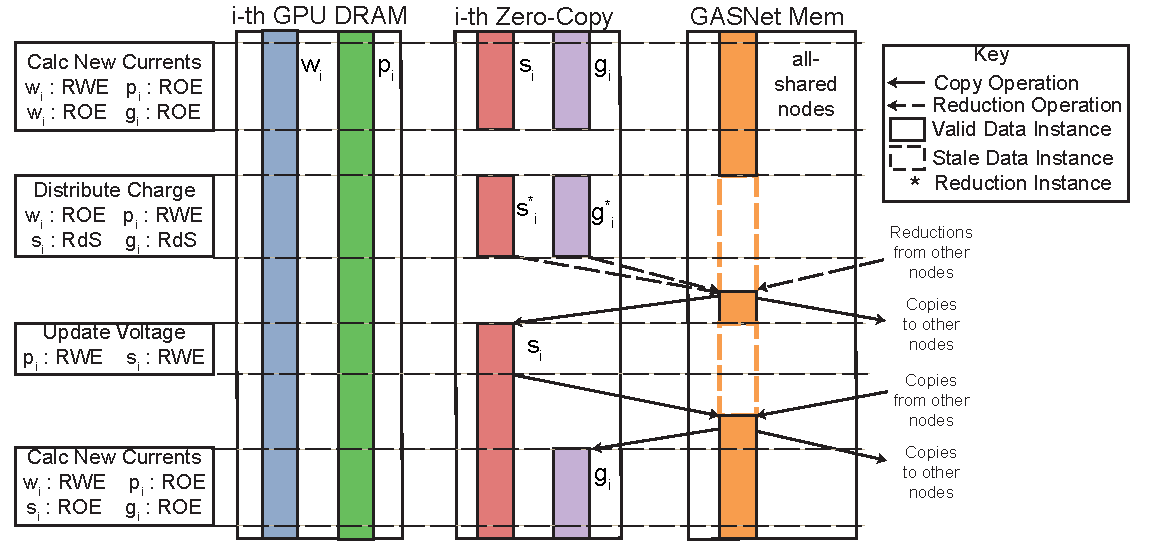
\includegraphics[scale=0.48]{figs/CircuitMem.pdf}
\caption{Tasks and data for the circuit simulation on a cluster of GPUs.}
\label{fig:gpumapping}
\end{figure}

\subsection{Execution}
\label{sec:exec}

Once a task $t$ has been mapped it enters the execution stage of the SOOP.  When all of
the operations (other tasks and copies) on which $t$ depends have completed, $t$ is
launched on the processor.  When $t$ launches subtasks, they are recursively scheduled as siblings by
the SOOP using $t$ as the parent task and $t$'s region arguments as the roots of the region forest.


\subsection{Clean-Up}
\label{sec:clean}

Once a task is done executing the various pieces of state associated with it can be reclaimed.
Dependence and mapping information can be removed from the region tree; in point of fact, 
as an optimization we are often able to remove tasks from the region tree well before the task terminates.
The most involved aspect of clean-up is colleting physical instances that are no longer in use.
We use a distributed reference counting scheme to track the number of tasks using physical instances;
when this number goes to 0 the physical intance can be reclaimed.


